% !TEX TS-program = knitr
\documentclass[handout]{beamer}\usepackage[]{graphicx}\usepackage[]{color}
% maxwidth is the original width if it is less than linewidth
% otherwise use linewidth (to make sure the graphics do not exceed the margin)
\makeatletter
\def\maxwidth{ %
  \ifdim\Gin@nat@width>\linewidth
    \linewidth
  \else
    \Gin@nat@width
  \fi
}
\makeatother

\definecolor{fgcolor}{rgb}{0.345, 0.345, 0.345}
\newcommand{\hlnum}[1]{\textcolor[rgb]{0.686,0.059,0.569}{#1}}%
\newcommand{\hlstr}[1]{\textcolor[rgb]{0.192,0.494,0.8}{#1}}%
\newcommand{\hlcom}[1]{\textcolor[rgb]{0.678,0.584,0.686}{\textit{#1}}}%
\newcommand{\hlopt}[1]{\textcolor[rgb]{0,0,0}{#1}}%
\newcommand{\hlstd}[1]{\textcolor[rgb]{0.345,0.345,0.345}{#1}}%
\newcommand{\hlkwa}[1]{\textcolor[rgb]{0.161,0.373,0.58}{\textbf{#1}}}%
\newcommand{\hlkwb}[1]{\textcolor[rgb]{0.69,0.353,0.396}{#1}}%
\newcommand{\hlkwc}[1]{\textcolor[rgb]{0.333,0.667,0.333}{#1}}%
\newcommand{\hlkwd}[1]{\textcolor[rgb]{0.737,0.353,0.396}{\textbf{#1}}}%
\let\hlipl\hlkwb

\usepackage{framed}
\makeatletter
\newenvironment{kframe}{%
 \def\at@end@of@kframe{}%
 \ifinner\ifhmode%
  \def\at@end@of@kframe{\end{minipage}}%
  \begin{minipage}{\columnwidth}%
 \fi\fi%
 \def\FrameCommand##1{\hskip\@totalleftmargin \hskip-\fboxsep
 \colorbox{shadecolor}{##1}\hskip-\fboxsep
     % There is no \\@totalrightmargin, so:
     \hskip-\linewidth \hskip-\@totalleftmargin \hskip\columnwidth}%
 \MakeFramed {\advance\hsize-\width
   \@totalleftmargin\z@ \linewidth\hsize
   \@setminipage}}%
 {\par\unskip\endMakeFramed%
 \at@end@of@kframe}
\makeatother

\definecolor{shadecolor}{rgb}{.97, .97, .97}
\definecolor{messagecolor}{rgb}{0, 0, 0}
\definecolor{warningcolor}{rgb}{1, 0, 1}
\definecolor{errorcolor}{rgb}{1, 0, 0}
\newenvironment{knitrout}{}{} % an empty environment to be redefined in TeX

\usepackage{alltt}

\usetheme{Marburg}
\setbeamertemplate{navigation symbols}{} 
\setbeamertemplate{footline}
{
  \leavevmode%
  \hbox{%
  \begin{beamercolorbox}[wd=.333333\paperwidth,ht=2.25ex,dp=1ex,center]{author in head/foot}%
    \usebeamerfont{author in head/foot} $\ $ \insertshortauthor%~~\beamer@ifempty{\insertshortinstitute}{}{(\insertshortinstitute)}
  \end{beamercolorbox}%
  \begin{beamercolorbox}[wd=.333333\paperwidth,ht=2.25ex,dp=1ex,center]{title in head/foot}%
    \usebeamerfont{title in head/foot} \insertinstitute
  \end{beamercolorbox}%
  \begin{beamercolorbox}[wd=.333333\paperwidth,ht=2.25ex,dp=1ex,right]{date in head/foot}%
    \usebeamerfont{date in head/foot}\insertshortdate{}\hspace*{2em}
    \insertframenumber{} / \inserttotalframenumber\hspace*{2ex} 
  \end{beamercolorbox}}%
  \vskip0pt%
}

\usepackage{amsmath}
\usepackage{caption}
\usepackage{color}
\usepackage{enumerate}
\usepackage{listings}
\usepackage{hyperref}
\usepackage{mathrsfs}
\usepackage{natbib}
\usepackage{url}

\providecommand{\all}{\ \forall \ }
\providecommand{\bs}{\backslash}
\providecommand{\e}{\varepsilon}
\providecommand{\E}{\ \exists \ }
\providecommand{\lm}[2]{\lim_{#1 \rightarrow #2}}
\providecommand{\m}[1]{\mathbb{#1}}
\providecommand{\nv}{{}^{-1}}
\providecommand{\ov}[1]{\overline{#1}}
\providecommand{\p}{\newpage}
\providecommand{\q}{$\quad$ \newline}
\providecommand{\rt}{\rightarrow}
\providecommand{\Rt}{\Rightarrow}
\providecommand{\vc}[1]{\boldsymbol{#1}}
\providecommand{\wh}[1]{\widehat{#1}}

\hypersetup{colorlinks,linkcolor=,urlcolor=blue}
\numberwithin{equation}{section}

\definecolor{dkgreen}{rgb}{0,0.6,0}
\definecolor{gray}{rgb}{0.5,0.5,0.5}
\definecolor{mauve}{rgb}{0.58,0,0.82}

\lstset{ 
  language=C,                % the language of the code
  basicstyle= \footnotesize,           % the size of the fonts that are used for the code
  numberstyle= \tiny \color{white},  % the style that is used for the line-numbers
  stepnumber=2,                   % the step between two line-numbers. 
  numbersep=5pt,                  % how far the line-numbers are from the code
  backgroundcolor=\color{white},      % choose the background color. You must add \usepackage{color}
  showspaces=false,               % show spaces adding particular underscores
  showstringspaces=false,         % underline spaces within strings
  showtabs=false,                 % show tabs within strings adding particular underscores
  frame=lrb,                   % adds a frame around the code
  rulecolor=\color{black},        % if not set, the frame-color may be changed on line-breaks within not-black text 
  tabsize=2,                      % sets default tabsize to 2 spaces
  captionpos=t,                   % sets the caption-position 
  breaklines=true,                % sets automatic line breaking
  breakatwhitespace=false,        % sets if automatic breaks should only happen at whitespace
  %title=\lstname,                   % show the filename of files included with \lstinputlisting;
  keywordstyle=\color{blue},          % keyword style
  commentstyle=\color{gray},       % comment style
  stringstyle=\color{dkgreen},         % string literal style
  escapeinside={\%*}{*)},            % if you want to add LaTeX within your code
  morekeywords={*, ...},               % if you want to add more keywords to the set
  xleftmargin=0.053in, % left horizontal offset of caption box
  xrightmargin=-.03in % right horizontal offset of caption box
}

%\DeclareCaptionFont{white}{\color{white}}
%\DeclareCaptionFormat{listing}{\parbox{\textwidth}{\colorbox{gray}{\parbox{\textwidth}{#1#2#3}}\vskip-0.05in}}
%\captionsetup[lstlisting]{format = listing, labelfont = white, textfont = white}
%For caption-free listings, comment out the 3 lines above and uncomment the 2 lines below.
 \captionsetup{labelformat = empty, labelsep = none}
 \lstset{frame = single}



\title{Inference for Unstructured Multisample Studies (Ch. 7.1, 7.2, 7.4)}
\author{Yifan Zhu}
\date{}
\institute{Iowa State University}
\IfFileExists{upquote.sty}{\usepackage{upquote}}{}
\begin{document}

\begin{frame}
\titlepage
 \end{frame}
 
 \AtBeginSection[]
{
   \begin{frame}
       \frametitle{Outline}
       \tableofcontents[currentsection]
   \end{frame}
}

\section{The one-way ANOVA model}

\begin{frame}
\frametitle{The one-way ANOVA model}
\begin{itemize}
\item Suppose we have:
\begin{itemize}
\pause \item Some response variable, $Y$
\pause \item Some covariate factor, $X$, with levels $i = 1, 2, \ldots, r$ and $n_i$ observations at level $i$.
\end{itemize}
\pause \item The {\bf one-way ANOVA model}, sometimes called the one-way normal model, is:
\pause \begin{align*}
Y_{ij} = \mu_{i} + \e_{ij}
\end{align*}
where:
\begin{itemize}
\pause \item The $\e_{ij}$'s are iid $N(0,\sigma^2)$
\pause \item $\mu_i$ is the true mean response at level $i$ of the factor.
\pause \item $j = 1, 2, \ldots, n_i$.
\end{itemize}
\end{itemize}
\end{frame}


\begin{frame}
\frametitle{The one-way ANOVA model}
 \begin{align*}
Y_{ij} = \mu_i + \e_{ij}
\end{align*}
\begin{center}
\setkeys{Gin}{width=1\textwidth} 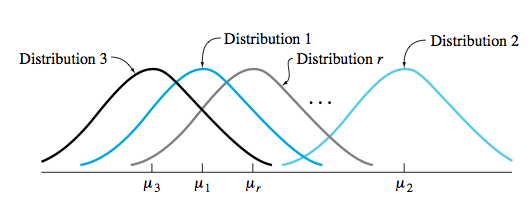
\includegraphics{../../fig/modelsnormal.png}
\end{center}
\end{frame}



\begin{frame}
\frametitle{Example: concrete}
\begin{itemize}
\item Compressive strengths of 8 different formulas of concrete:
\begin{center}
\setkeys{Gin}{width=.7\textwidth} 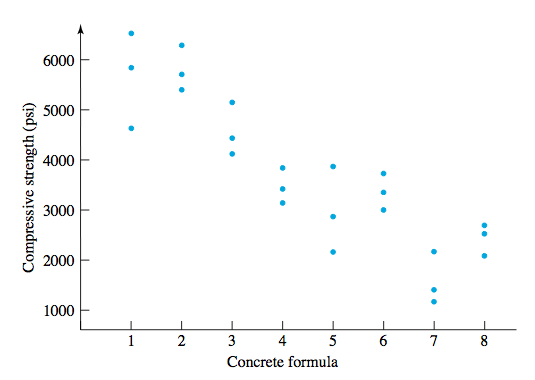
\includegraphics{../../fig/concreteplot.png}
\end{center}
\pause \item But the order of the numbers given to the formulas is meaningless. It wouldn't make sense to do a simple linear regression of strength on formula.
\end{itemize}
\end{frame}

\begin{frame}
\frametitle{Example: concrete}
\begin{itemize}
\item Instead of:
\pause \begin{align*}
Y_i = \beta_0 + \beta_1 X_i + \e_i
\end{align*}
\pause with $Y_i$ as strength and $X_i$ as the formula index, we use:
\pause \begin{align*}
Y_{ij} = \mu_{i} + \e_{ij}
\end{align*}
where:
\begin{itemize}
\pause \item $i$ is the formula index, $i = 1, 2, \ldots, 8$
\pause \item $j$ is the index of a specimen within the formula $i$ group.
\end{itemize}
\end{itemize}
\end{frame}

\begin{frame}
\frametitle{Example: springs}
\begin{itemize}
\item Spring constants of three types of steel springs:
\end{itemize}
\begin{center}
\setkeys{Gin}{width=.7\textwidth} 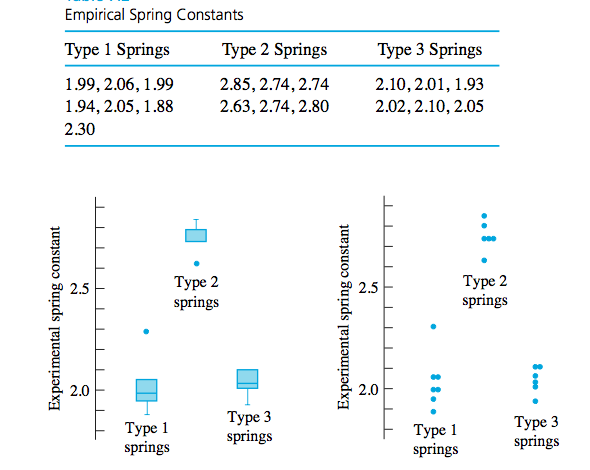
\includegraphics{../../fig/springconst.png}
\end{center}
\end{frame}

\begin{frame}
\frametitle{Example: springs}
\begin{itemize}
\item Doesn't make sense to regress exponential spring constant on spring type.
\pause \item Instead, we apply:
\begin{align*}
Y_{ij} = \mu_{i} + \e_{ij}
\end{align*}
where:
\begin{itemize}
\pause \item $Y_{ij}$ is the exponential spring constant of spring type $i$ spring number $j$.
\pause \item $\mu_{i}$ is the true mean exponential spring constant of type $i$.
\pause \item $i$ is the formula index, $i = 1, 2, \ldots, 8$
\pause \item $j$ is the index of a specimen within the formula $i$ group.
\end{itemize}
\end{itemize}
\end{frame}

\section{Residuals and fitted values}

\begin{frame}
\frametitle{Fitted values} \small
\begin{itemize}
\item Similarly to before, $\wh{y}_{ij}$ is the fitted value corresponding to $y_{ij}$. It represents an estimate of the true mean response at factor level $i$ and sample unit $j$.
\pause \item We treat all sample units equally, letting;
\pause \begin{align*}
\wh{y}_{ij} = \hat{\mu}_i =\ov{y}_{i.} = \frac{1}{n_i} \sum_{j=1}^{n_i} y_{ij}
\end{align*}
\pause the average of all the responses at factor level $i$.
\pause \item We get $\wh{\mu}_{i} = \ov{y}_{i.}$ by minimizing the loss function:
\pause \begin{align*}
S(\mu_1, \mu_2, \ldots, \mu_r) = \sum_{ij}(y_{ij} - \mu_i)^2
\end{align*}
over all the choices of $\mu_1, \mu_2, \ldots, \mu_r$, selecting $\ov{y}_{i.}$ to estimate $\mu_i$. 
\pause \item The residuals $e_{ij}$ are then:
\begin{align*}
e_{ij} = y_{ij} - \ov{y}_{i.}
\end{align*}
\end{itemize}
\end{frame}



\begin{frame}
\frametitle{Example: concrete}
\begin{center}
\setkeys{Gin}{width=1\textwidth} 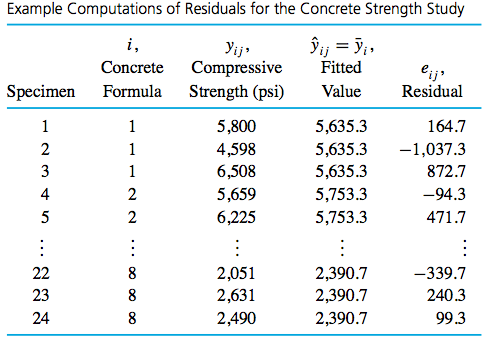
\includegraphics{../../fig/concreteresd.png}
\end{center}
\end{frame}

\begin{frame}
\frametitle{Example: concrete}
\begin{center}
\setkeys{Gin}{width=1\textwidth} 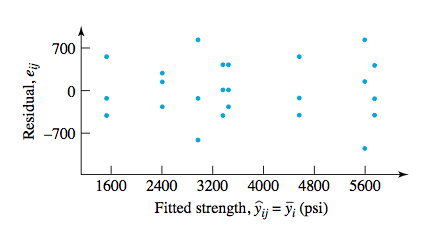
\includegraphics{../../fig/concreteres2.png}
\end{center}
\end{frame}

\begin{frame}
\frametitle{Example: concrete}
\begin{center}
\setkeys{Gin}{width=1\textwidth} 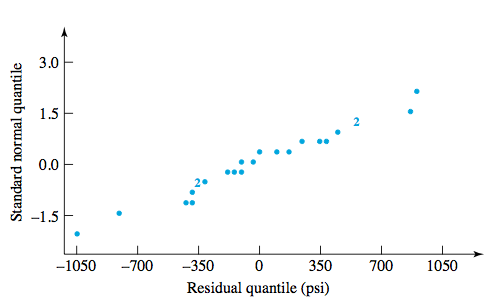
\includegraphics{../../fig/concreteres3.png}
\end{center}
\end{frame}

\section{Variance estimation}


\begin{frame}
\frametitle{Variance estimation}
\begin{itemize}
\item We can compute a sample variance for each factor level:
\begin{align*}
s_i^2 = \frac{1}{n_i - 1}  \sum_j (y_{ij} - \ov{y}_{ij})^2
\end{align*}
\pause \item And we can compute a {\bf pooled sample variance}:
\begin{align*}
s_P^2 = \frac{(n_1 - 1)s_1^2 + (n_2 - 1)s_2^2 + \cdots + (n_r - 1)s_r^2}{(n_1 - 1) + (n_2 - 1) + \cdots + (n_r - 1)} \\
\end{align*}
\pause \item The pooled sample standard deviation is just $s_P = \sqrt{s_P^2}$
\end{itemize}
\end{frame}

\begin{frame}
\frametitle{Variance estimation} \scriptsize
\begin{itemize}
\item If $n = \sum_i n_i$, then:

\begin{align*}
s_P^2 &= \frac{(n_1 - 1)s_1^2 + (n_2 - 1)s_2^2 + \cdots + (n_r - 1)s_r^2}{(n_1 - 1) + (n_2 - 1) + \cdots + (n_r - 1)} \\
&\uncover<2->{= \frac{(n_1 - 1) \left (\frac{1}{n_1 - 1}\right ) \sum_j (y_{1j} - \ov{y}_1)^2 + \cdots + (n_r - 1) \left (\frac{1}{n_r - 1}\right ) \sum_j (y_{lj} - \ov{y}_l)^2}{n - r}} \\
&\uncover<3->{= \frac{1}{n-r} \sum_{ij} (y_{ij} - \ov{y}_i)^2} \\
&\uncover<4->{= \frac{1}{n - r} \sum_{ij} e_{ij}^2}
\end{align*}
\uncover<5->{\item As it turns out, }
\begin{align*}
\uncover<5->{E(s_P^2)} & \uncover<5->{= \sigma^2} \\
\uncover<6->{\frac{n-r}{\sigma^2} s_P^2}& \uncover<6->{ \sim \chi^2_{n - r}}
\end{align*}
\uncover<7->{\item A $1 - \alpha$ confidence interval for $\sigma^2$ is of the form: }
\begin{align*}
\uncover<8->{\left ( \frac{n-r}{\chi^2_{n - r, \ 1 - \alpha/2}}s^2_P, \ \frac{n-r}{\chi^2_{n - r , \ \alpha/2}}s^2_P  \right )}
\end{align*}
\end{itemize}
\end{frame}

\begin{frame}
\frametitle{Example: concrete}
\begin{center}
\setkeys{Gin}{width=1\textwidth} 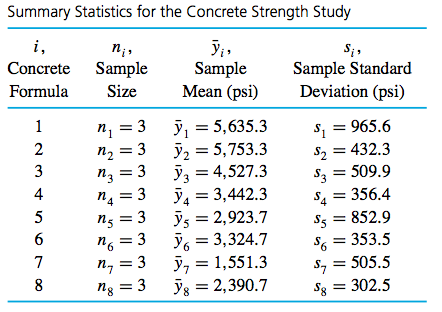
\includegraphics{../../fig/concindivsd.png}
\end{center}
\end{frame}

\begin{frame}
\frametitle{Example: concrete} \small
\begin{align*}
\uncover<1->{s_P^2} & \uncover<1->{= \frac{(3-1)(965.6)^2 + (3-1)(432.3)^2 + \cdots + (3-1)(302.5)^2}{(3 -1 ) + \cdots + (3-1)}} \\
&\uncover<2->{=2 \frac{965.6^2 + 432.3^2 + \cdots + 302.5^2}{16}} \\
&\uncover<3->{= 338213 \text{ psi}^2} \\
\uncover<4->{s_P} &\uncover<4->{= \sqrt{338213}} \uncover<5->{= 581.6 psi}
\end{align*}

\end{frame}

\begin{frame}
\frametitle{Example: concrete}
\begin{itemize}
\item $n = 24$, $r = 8$, $n-r = 16$.
\pause \item $\chi^2_{16, \ 0.95} = 26.296$, $\chi^2_{16, \ 0.05} = 7.962$
\pause \item Hence, a 90\% 2-sided confidence interval for $\sigma^2$ is:
\pause \begin{align*}
\left ( \frac{16 \cdot 581.6^2}{26.296}, \ \frac{16 \cdot 581.6^2}{7.962} \right ) \\
&= (205816, \ 679745.9)
\end{align*}
\pause and you can make a 90\% confidence interval for $\sigma$ by transforming the endpoints of the confidence interval for $\sigma^2$:
\pause \begin{align*}
 (\sqrt{205816}, \ \sqrt{679745.9}) = (453.7, \ 824.5)
\end{align*}
\pause \item We're 90\% confident that the true overall standard deviation of compressive strength of the concrete within factor levels is between 453.7 psi and 824.5 psi.
\end{itemize}
\end{frame}


\section{Standardized residuals}
\begin{frame}
\frametitle{Standardized residuals}
\begin{itemize}
\item Just as before, even though $\e_{ij} \sim $ iid N($0, \sigma^2$), the $e_{ij}$'s don't have constant variance.
\pause \item The {\bf standardized residuals} for the one-way ANOVA model are of the form:
\pause \begin{align*}
e_{ij}^* = \frac{e_{ij}}{s_P \sqrt{\frac{n_i - 1}{n_i}}}
\end{align*}
which are approximately $N(0,1)$.
\end{itemize}
\end{frame}


\section{Inference}


\begin{frame}
\frametitle{Inference for the one-way ANOVA model}
\begin{enumerate}[1. ]
\item $H_0: \mu_1 = \mu_2 = \cdots = \mu_r$, $H_a:$ not all the $\mu_i$'s are equal.
\pause \item $\alpha$ is some sensible value.
\pause \item The test statistic is:
\pause \begin{align*}
F = \frac{MSR}{MSE} = \frac{SSR/(r-1)}{SSE/(n-r)}
\end{align*}
\begin{itemize}
\item Here,
\begin{itemize}
\pause \item $n$ is the number of observations.
\pause \item $r$ is the number of levels of the covariate.
\pause \item $SSR = \sum_{ij} (\wh{y}_{ij} - \ov{y}_{..})^2 = \sum_{ij} (\ov{y}_{i.} - \ov{y}_{..})^2 $
\pause \item $SSE = \sum_{ij} ({y_{ij} - \wh{y}_{ij}})^2 = \sum_{ij} (y_{ij} - \ov{y}_{i.})^2$
% \pause \item $SST = \sum_{ij} (y_{ij} - \ov{y}_{..})^2 $
% \pause \item $\ov{y}_{..} = \frac{1}{n} \sum_{ij} y_{ij}$
\end{itemize}
\pause \item Assume $H_0$ is true, the model is valid, and the $\e_{ij}$'s are iid $N(0, \sigma^2)$
\pause \item Then, $F \sim F_{r -1, \ n - r}$. 
\pause \item Reject $H_0$ if $F > F_{r - 1, \ n - r, \ 1 - \alpha}$
\end{itemize}
\end{enumerate}
\end{frame}

\begin{frame}
\frametitle{Inference for the one-way ANOVA model}
\begin{enumerate}
\setcounter{enumi}{3}
\item Compute the observed $F$ using data. To do that, we can construct the ANOVA table: \q
\begin{center}
\pause \begin{tabular}{lllll}
Source & SS & df & MS & F  \\ \hline
Covariate & SSR & $r-1$ & $SSR/(r-1)$ & MSR/MSE \\ 
Error & SSE & $n-l$ & $SSE/(n-r)$ & 
\end{tabular}
\end{center}
\item If $observed F >  F_{r-1, n-r, 1 - \alpha}$, reject $H_0$; or we can compute the p-value: 
\[P(F_{r-1, n-r} > observed F)\]
If the p-value is small, we reject $H_0$.
\item
Conclusion in layman's term.
\end{enumerate}
\end{frame}


\begin{frame}
\frametitle{Example: concrete}
\begin{enumerate}[1. ]
\item $H_0: \mu_1 = \mu_2 = \cdots = \mu_8$, $H_a:$ not all the $\mu_i$'s are equal.
\pause \item $\alpha = 0.05$
\pause \item The test statistic is:
\pause \begin{align*}
F = \frac{MSR}{MSE} = \frac{SSR/(r-1)}{SSE/(n-r)} = \frac{SSR/7}{SSE/16}
\end{align*}
\begin{itemize}
\pause \item Assume $H_0$ is true, the model is valid, and the $\e_{ij}$'s are iid $N(0, \sigma^2)$
\pause \item Then, $F \sim F_{r -1, \ n - r}$. 
\pause \item Reject $H_0$ if $F > F_{r - 1, \ n - r, \ 1 - \alpha} = F_{7, 16, 0.95} = 2.66$
\end{itemize}
\end{enumerate}
\end{frame}



\begin{frame}
\frametitle{Example: concrete}
\begin{enumerate}
\setcounter{enumi}{3}
\item We start by calculating $SST, s^2_P$, and $SSE$:
\begin{center}
\setkeys{Gin}{width=.8\textwidth} 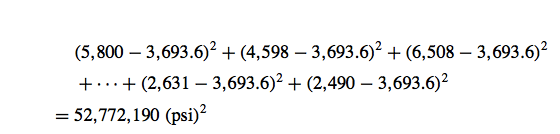
\includegraphics{../../fig/conc1.png}
\setkeys{Gin}{width=.6\textwidth} 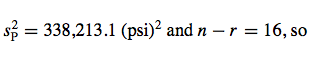
\includegraphics{../../fig/conc2.png}
\setkeys{Gin}{width=.6\textwidth} 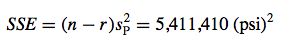
\includegraphics{../../fig/conc3.png}
\end{center}
Lastly, we calculate $SSR$:
\begin{center}
\setkeys{Gin}{width=.5\textwidth} 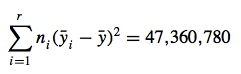
\includegraphics{../../fig/conc4.png}
\end{center}
\end{enumerate}
\end{frame}

\begin{frame}
\frametitle{Example: concrete}
\begin{center}
\setkeys{Gin}{width=.8\textwidth} 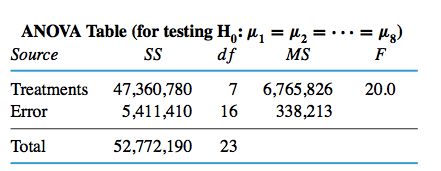
\includegraphics{../../fig/conc5.png}
\end{center}
\begin{enumerate}
\setcounter{enumi}{4}
\item With $observedF = 20.0 > 2.66$, we reject $H_0$ and conclude $H_a$.
\item There is enough evidence to conclude that the compressive strength of the concrete varies with formula.
\end{enumerate}
\end{frame}


\begin{frame}
\frametitle{Example: railroad rails} \small
\begin{itemize}
\item The following data are taken from the paper \emph{Zero- Force Travel-Time Parameters for Ultrasonic Head-Waves in Railroad Rail} by Bray and Leon- Salamanca (Materials Evaluation, 1985).
\pause \item Given are measurements in nanoseconds of the travel time (in excess of 36.1 $\mu s$) of a certain type of mechanical wave induced by mechanical stress in railroad rails. 
\begin{center}
\setkeys{Gin}{width=.6\textwidth} 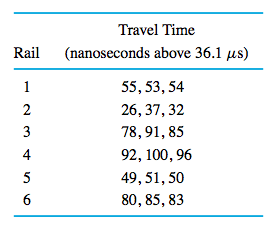
\includegraphics{../../fig/railsdat.png}
\end{center}
\end{itemize}
\end{frame}

\begin{frame}
\frametitle{Example: railroad rails}
\begin{itemize}
\item We apply the model:
\pause \begin{align*}
Y_{ij} = \mu_{i} + \e_{ij}
\end{align*}
where:
\begin{itemize}
\pause \item $Y_{ij}$ is the observed travel time (ns) of the wave in excess of 26.1 $\mu s$ for Rail $i$ wave $j$.
\pause \item $\mu_i$ is the true mean travel time (ns) in excess of 26.1 $\mu s$ of waves through Rail $i$.
\end{itemize}
\end{itemize}
\end{frame}



\begin{frame}
\frametitle{Example: railroad rails}
\begin{center}
\setkeys{Gin}{width=1\textwidth} 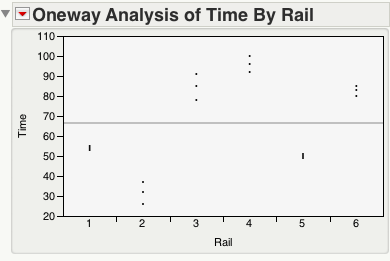
\includegraphics{../../fig/railplot.png}
\end{center}
\end{frame}

\begin{frame}
\frametitle{Example: railroad rails}
\begin{center}
\setkeys{Gin}{width=0.9\textwidth} 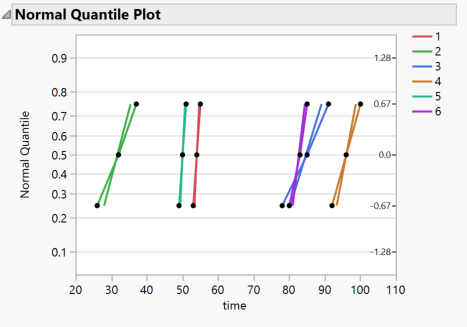
\includegraphics{../../fig/rails_QQ.png}
\end{center}
\end{frame}

\begin{frame}
\frametitle{Example: railroad rails}
\begin{center}
\setkeys{Gin}{width=1\textwidth} 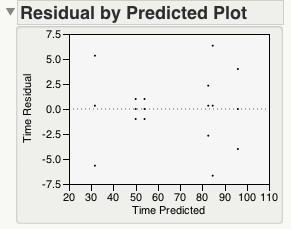
\includegraphics{../../fig/railresid.png}
\end{center}
\end{frame}

\begin{frame}
\frametitle{Example: railroad rails}
\begin{center}
\setkeys{Gin}{width=0.9\textwidth} 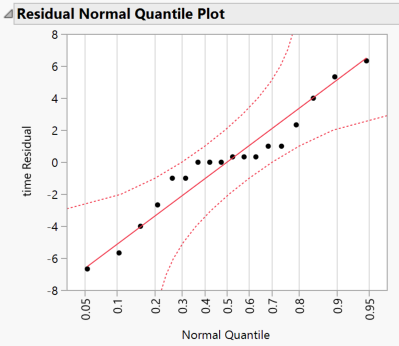
\includegraphics{../../fig/rails_res_QQ.png}
\end{center}
\end{frame}







\begin{frame}
\frametitle{Example: railroad rails}
\begin{enumerate}[1. ]
\item $H_0: \mu_1 = \mu_2 = \cdots = \mu_6$, $H_a:$ not all the $\mu_i$'s are equal.
\pause \item $\alpha = 0.05$
\pause \item The test statistic is:
\begin{align*}
\uncover<4->{F = \frac{MSR}{MSE}} \uncover<5->{ = \frac{SSR/(r-1)}{SSE/(n-r)}} \uncover<6->{ = \frac{SSR/(6-1)}{SSE/(18-6)} } \uncover<7->{= \frac{SSR/5}{SSE/12}}
\end{align*}
\begin{itemize}
\uncover<8->{\item Assume $H_0$ is true, the model is valid, and the $\e_{ij}$'s are iid $N(0, \sigma^2)$}
\uncover<9->{\item Then, $F \sim F_{r -1, \ n - r}$.}
\uncover<10->{\item Reject $H_0$ if $F > F_{r - 1, \ n - r, \ 1 - \alpha} = F_{5, 12, 0.95} = 3.11$}
\end{itemize}
\end{enumerate}
\end{frame}


\begin{frame}
\frametitle{Example: railroad rails}
\begin{enumerate}
\setcounter{enumi}{3}
\item Load the data into JMP and fit travel time on rail, and \emph{make sure the rail variable is a factor}.
\end{enumerate}
\begin{center}
\setkeys{Gin}{width=1\textwidth} 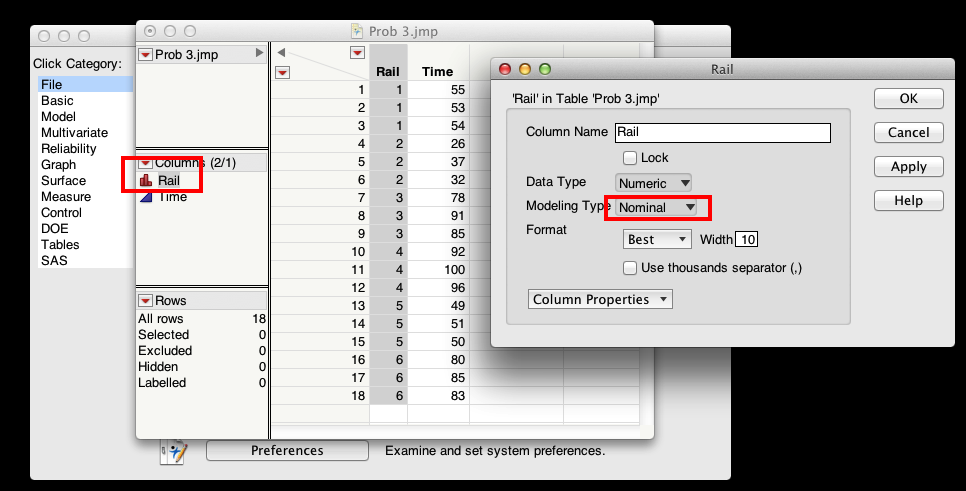
\includegraphics{../../fig/nominalrail.png}
\end{center}
\end{frame}


\begin{frame}
\frametitle{Example: railroad rails}
\begin{center}
\setkeys{Gin}{width=.8\textwidth} 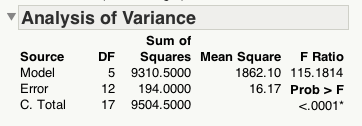
\includegraphics{../../fig/railanova.png}
\end{center}
\begin{enumerate}[1. ]
\setcounter{enumi}{4}
\item With $observedF = 115.18 > 3.11$, we reject $H_0$ and conclude $H_a$.
\pause \item There is enough evidence to conclude that the true mean excess travel time of waves along the rails depends on the rail.
\end{enumerate}
\end{frame}

\section{Confidence interval for linear combination of means}

\begin{frame}
\frametitle{Confidence interval for linear combination of means}
\begin{itemize}
\item
When we have multiple samples with means $\mu_1, \mu_2, \ldots, \mu_r$, we want to compare these means
\item
There are many possibilities: $\mu_1$, $\mu_1 - \mu_2,\, \mu_1 - \mu_2, \frac{1}{2}(\mu_1 + \mu_2) - \mu_3 \ldots$.
\item
We will construct a confidence interval for a linear combination of these means. We denote the linear combination as
\[L = c_1 \mu_1 + c_2 \mu_2 + \cdots + c_r \mu_r\]
\end{itemize}
\end{frame}

\begin{frame}
\frametitle{Confidence interval for linear combination of means}
\begin{itemize}
\item
Since the estimate for $\mu_i$ is $\bar{y}_{i\cdot}$, the estimate of $L$ is 
\[\hat{L} = c_1 \bar{y}_{1\cdot} + c_2 \bar{y}_{2\cdot} + \cdots + c_r \bar{y}_{r\cdot}\]

\item
Under the one-way normal model, $\bar{y}_{i\cdot} \sim N(\mu_i, \sigma^2/n_i)$. So 
\begin{align*}
\hat{L} \sim N\bigg(&c_1 \mu_1 + c_2 \mu_2 + \cdots + c_r \mu_r,\\
&\sigma^2 \left(\frac{c_1^2}{n_1} + \frac{c_2^2}{n_2} + \cdots + \frac{c_r^2}{n_r}\right) \bigg)
\end{align*}
\end{itemize}
\end{frame}
\begin{frame}
\frametitle{Confidence interval for linear combination of means}
\begin{itemize}
\item
Thus
\[\frac{\hat{L} - L}{\sigma\sqrt{\frac{c_1^2}{n_1} + \frac{c_2^2}{n_2} + \cdots + \frac{c_r^2}{n_r}}} \sim N(0,1)\]
\item
Replacing the unknown $\sigma$ with the pooled sample standard deviation, then
\[\frac{\hat{L} - L}{s_P\sqrt{\frac{c_1^2}{n_1} + \frac{c_2^2}{n_2} + \cdots + \frac{c_r^2}{n_r}}} \sim t_{n-r}\]
\item 
Therefore a two-sided $1-\alpha$ confidence interval is
\[\hat{L} \pm t_{n-r, 1 - \alpha/2} s_P \sqrt{\frac{c_1^2}{n_1} + \frac{c_2^2}{n_2} + \cdots + \frac{c_r^2}{n_r}}\]
The one-sidede confidence intervals are analogous.
\end{itemize}
\end{frame}
\begin{frame}
\frametitle{Example: railroad rails}
Construct the following confidence intervals with the JMP output:
\begin{enumerate}
\item 95\% two-sided confidence interval for $\mu_1$
\item 95\% two-sided confidence interval for $\mu_1 - \mu_2$
\item 95\% lower confidence bound for $\mu_3 - \mu_5$
\item 90\% two-sided confidence interval for $\frac{1}{2}(\mu_1 + \mu_2) - \mu_3$
\end{enumerate}
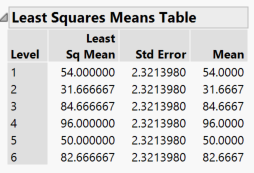
\includegraphics[width = 0.5\textwidth]{../../fig/rails_means.png}
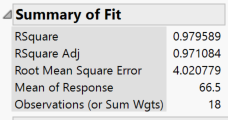
\includegraphics[width = 0.5\textwidth]{../../fig/rails_fit.png}
\end{frame}

\begin{frame}
\frametitle{Example: railroad rails}
\begin{itemize}
\item[1.]
$t_{n-r, 1 - \alpha/2} = t_{18 - 6, 1 - 0.05/2} = t_{12, 0.975} = 2.179$. So
\begin{align*}
&\bar{y}_{1\cdot}  \pm t_{12, 0.975} s_P \sqrt{\frac{1^2}{3}}\\ = & 54.000 \pm 2.179(4.021)\sqrt{1/3} \\
=& 54 \pm 5.059\\
= & (48.941, 59.059)
\end{align*}

We are 95\% confident that the mean mechanical wave travel time for Rail 1 is any number between 48.941 and 59.059 nanoseconds.
\end{itemize}
\end{frame}


\begin{frame}
\frametitle{Example: railroad rails}
\begin{itemize}
\item[2.]
$t_{n-r, 1 - \alpha/2} = t_{18 - 6, 1 - 0.05/2} = t_{12, 0.975} = 2.179$. So
\begin{align*}
&\bar{y}_{1\cdot} - \bar{y}_{2\cdot} \pm t_{12, 0.975} s_P \sqrt{\frac{1^2}{3} + \frac{(-1)^2}{3}}\\ = & (54.000 - 31.667) \pm 2.179(4.021)\sqrt{2/3} \\
=& 22.333 \pm 7.154 \\
= & (15.179, 29.487)
\end{align*}

We are 95\% confident that the mean mechanical wave travel time for Rail 1 is longer than that of Rail 2 by any number between 15.179 and 20.487 nanoseconds.
\end{itemize}
\end{frame}

\begin{frame}
\frametitle{Example: railroad rails}
\begin{itemize}
\item[3.]
$t_{n-r, 1 - \alpha} = t_{18 - 6, 1 - 0.05} = t_{12, 0.95} = 1.782$. So the lower 95\% confidence bound is
\begin{align*}
&\bar{y}_{3\cdot} - \bar{y}_{5\cdot} - t_{12, 0.95} s_P \sqrt{\frac{1^2}{3} + \frac{(-1)^2}{3}}\\ = & (84.667 - 50.000) \pm 1.782(4.021)\sqrt{2/3} \\
=&  34.667 - 5.851 \\
= & 28.816
\end{align*}

We are 95\% confident that the mean mechanical wave travel time for Rail 3 is longer than that of Rail 5 by at least 28.816 nanoseconds.
\end{itemize}
\end{frame}

\begin{frame}
\frametitle{Example: railroad rails}
\begin{itemize}
\item[4.]
$t_{n-r, 1 - \alpha/2} = t_{18 - 6, 1 - 0.1/2} = t_{12, 0.95} = 1.782$. So
\begin{align*}
&\frac{1}{2}\bar{y}_{1\cdot} + \frac{1}{2}\bar{y}_{2\cdot} - \bar{y}_{3\cdot} \pm t_{12, 0.95} s_P \sqrt{\frac{(1/2)^2}{3} + \frac{(1/2)^2}{3} + \frac{(-1)^2}{3}}\\ = & (\frac{1}{2}54.000 + \frac{1}{2}31.667 - 84.667) \pm 1.782(4.021)\sqrt{1/2} \\
=& -41.834 \pm 5.067 \\
= & (-46.901, -36.767)
\end{align*}

We are 90\% confident that the average of the mean mechanical wave travel times for Rail 1 and Rail 2 is shorter than the mean mechanical wave travel time of Rail 3 by any number between 46.901 and 36.767 nanoseconds.
\end{itemize}
\end{frame}
\end{document}
